

\section{Grundlagen}
In diesem Kapitel werden die verschiedenen Grundlagen für die Steuerungsarten erklärt.
\subsection{Phasenanschnittsteuerung}
Bei der Phasenanschnittsteuerung wird das Sinussignal über einen TRIAC geführt. Ein TRIAC sind zwei antiparallel geführt Thyristoren. Dieser zündet ab einem gewissen Zündimpuls nach jedem Nulldurchgang. Je später der TRIAC eingeschaltet wird, desto kleiner wird die mittlere Leistung über der Last. Ein Vorteil gegenüber einem Spannungsteiler ist, dass weniger Leistung gebraucht wird. Der Zündwinkel kann von 0\textdegree bis 180\textdegree gewählt werden, wobei bei 0\textdegree die maximale Leistung und bei 180\textdegree keine Leistung über der Last anliegt. Das Problem bei der Phasenanschnittsteuerung ist, dass diese Schaltung Oberwellen verursacht und so ungewünschte Effekte für den Netzbetreiber verursacht. Ein weiteres Problem betrifft den nicht-sinusförmigen Stromverlauf. Da Strom und Spannung nicht den gleichen Verlauf haben, tritt eine Verzerrungsblindleistung auf.  Der Strom verläuft zeitlich der Spannung nach wirkt so wie eine Induktivität. Deshalb wird dieses Verfahren vom EW nur bei kleinen Leistungen toleriert. Bei grossen Leistungen wird deshalb die Schwinungspaketsteuerung benutzt. In der Abbildung \ref{fig:Phasenanschnitt} ist erischtlich, wie der Phasenanschnitt bei einer Netzspannung aussieht. Grau gezeichnet ist die normale Netzspannung und rot ist die Spannung welcher an der Last anliegt. In dieser Abbildung wurde ein Winkel von 135\textdegree gewählt und somit ist die Leistung an der Last kleiner als mit der normalen Netzspannung. 

\begin{figure}[ht!]
	\centering
	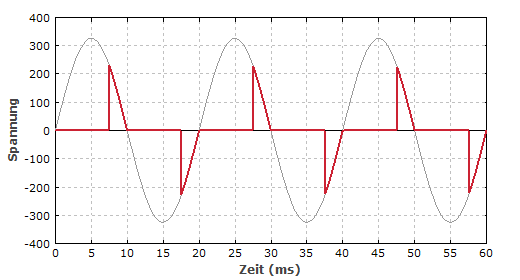
\includegraphics[scale=0.75]{phasenanschnittsteuerung1.png}	
	\caption{Phasenanschnitt mit einem Winkel von 135\textdegree \cite{Phasenanschnittsteuerung}}\label{fig:Phasenanschnitt1}
\end{figure}
\newpage
\begin{figure}[ht!]
	\centering
	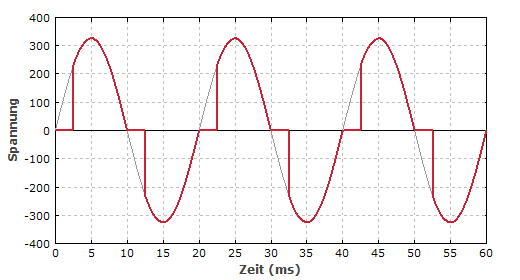
\includegraphics[scale=0.75]{phasenanschnittsteuerung2.png}	
	\caption{Phasenanschnitt mit einem Winkel von 45\textdegree \cite{Phasenanschnittsteuerung}}\label{fig:Phasenanschnitt2}
\end{figure}
Bei der Abbildung \ref{fig:Phasenanschnitt2} ist gut ersichtlich, wie früher gezündet wurde. Somit wird die Leistung an der Last grösser.

\subsection{Schwingungspaketsteuerung}
In diesem Verfahren wird nicht wie der Phasenanschnittsteuerung die Form der Halbwellen verändert, sondern die Zeitdauer. Dabei wird immer von der Paketzeit und der Einschaltzeit ausgegangen, wobei letzteres verändert wird. Wenn z.B. eine Paketdauer 10 Halbwellen hat, und die Einschaltdauer 5 Halbwellen ist, liegt die halbe Leistung über der Last an. Anders als bei der Phasenanschnittsteuerung enstehen bei dieser Ansteuerungsart keine harmonische Oberwellen, dafür aber Sub- und Zwischenharmonische. Auf der Abbildung \ref{fig:Schwingungspaketsteuerung} ist ersichtlicht, wie vier von den total sechs pro Paket eingeschaltet sind. Dies ergibt eine Leistung welche ${2}/{3}$ so gross ist wie die Leistung mit der normalen Netzspannung.

\begin{figure}[ht!]
	\centering
	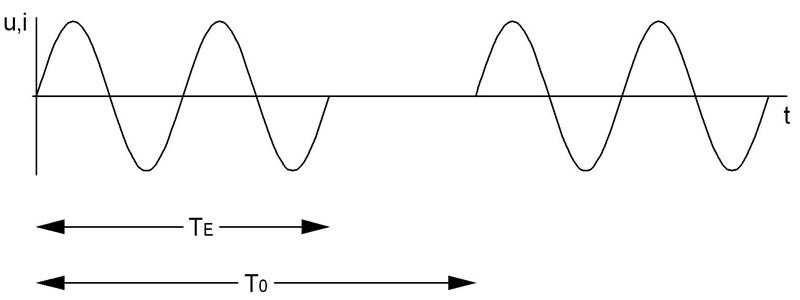
\includegraphics[scale=0.5]{Schwingungspaketsteuerung.png}	
	\caption{Schwingungspaketsteuerung ${2}/{3}$ der Leistung \cite{Schwingungspaketsteuerung}}\label{fig:Schwingungspaketsteuerung}
\end{figure}

Dabei ergibt sich aus dem Verhältnis von Einschaltdauer zu Periodendauer das Tastverhältnis.

\begin{equation}\label{eq:Einschaltverhältnis}
a = \frac{T_E}{T_0}
\end{equation}

\subsection{TRIAC}
Der TRIAC beseht aus zwei anti-parallele Thyristoren und kann über das Gate gezündet werden. Der TRIAC bleibt solange leitend bis der Haltestrom unterschritten wird. 

\begin{figure}[ht!]
	\centering
	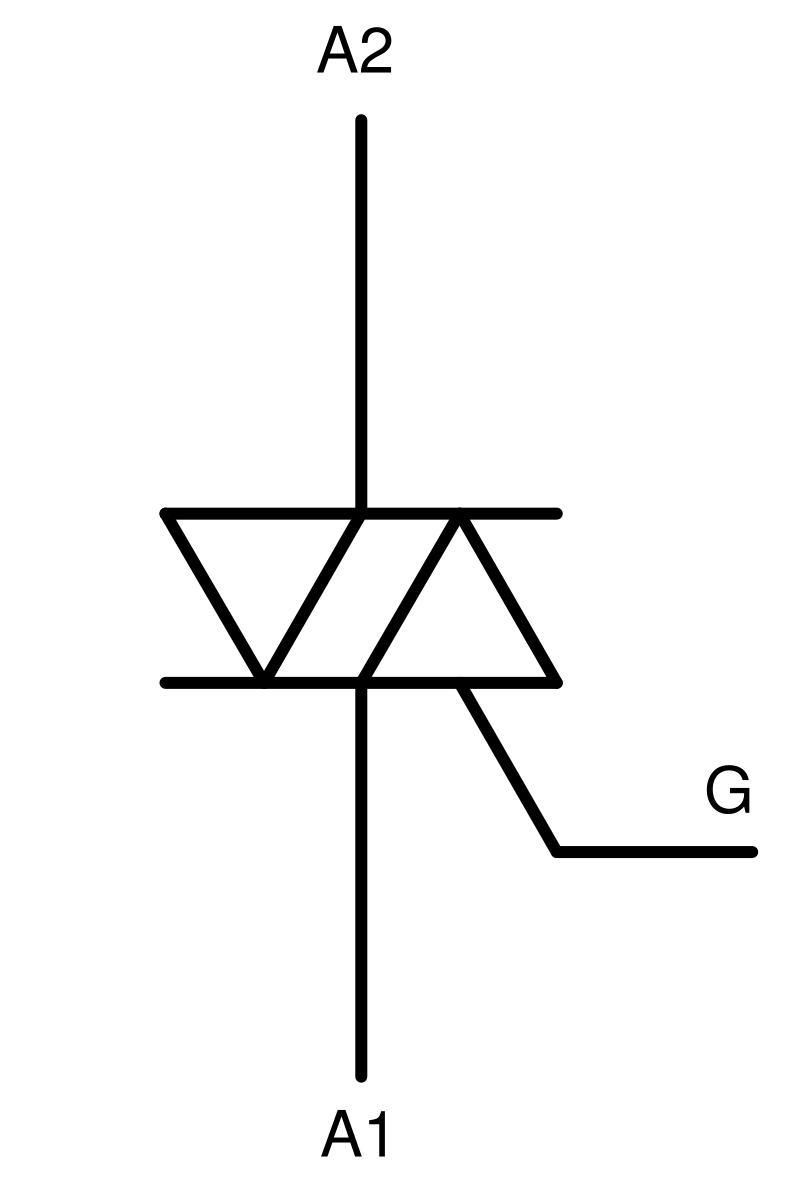
\includegraphics[scale=0.1]{TRIAC.png}	
	\caption{Schaltzeichen eines TRIACs \cite{TRIAC}}\label{fig:TRIAC}
\end{figure}




\subsection{Leistungsfaktor}
Bei beiden Verfahren ist der Leistungsfaktor vom Zündwinkel oder dem Einschaltverhältnis abhängig. 

In der Abbildung \ref{fig:Leistungsfaktor} ist ersichtlich wie der Leistungsfaktor bei den beiden Steuerungsarten aussieht. Bei der Phasenanschnittsteuerung auf der linken Seite sieht man, wie bei einem kleinem Zündwinkel der Leistungsfaktor sehr gross ist. Je grösser der Zündwinkel gewählt wird, desto kleiner wird der Leistungsfaktor. Auf der rechten Seite sieht man den Leistungsfaktor in Abhängigkeit des Einschaltverhältnisses. Je grösser das Einschaltzeitverhältnis, desto grösser der Leistungsfaktor.  
\begin{figure}[ht!]
	\centering
	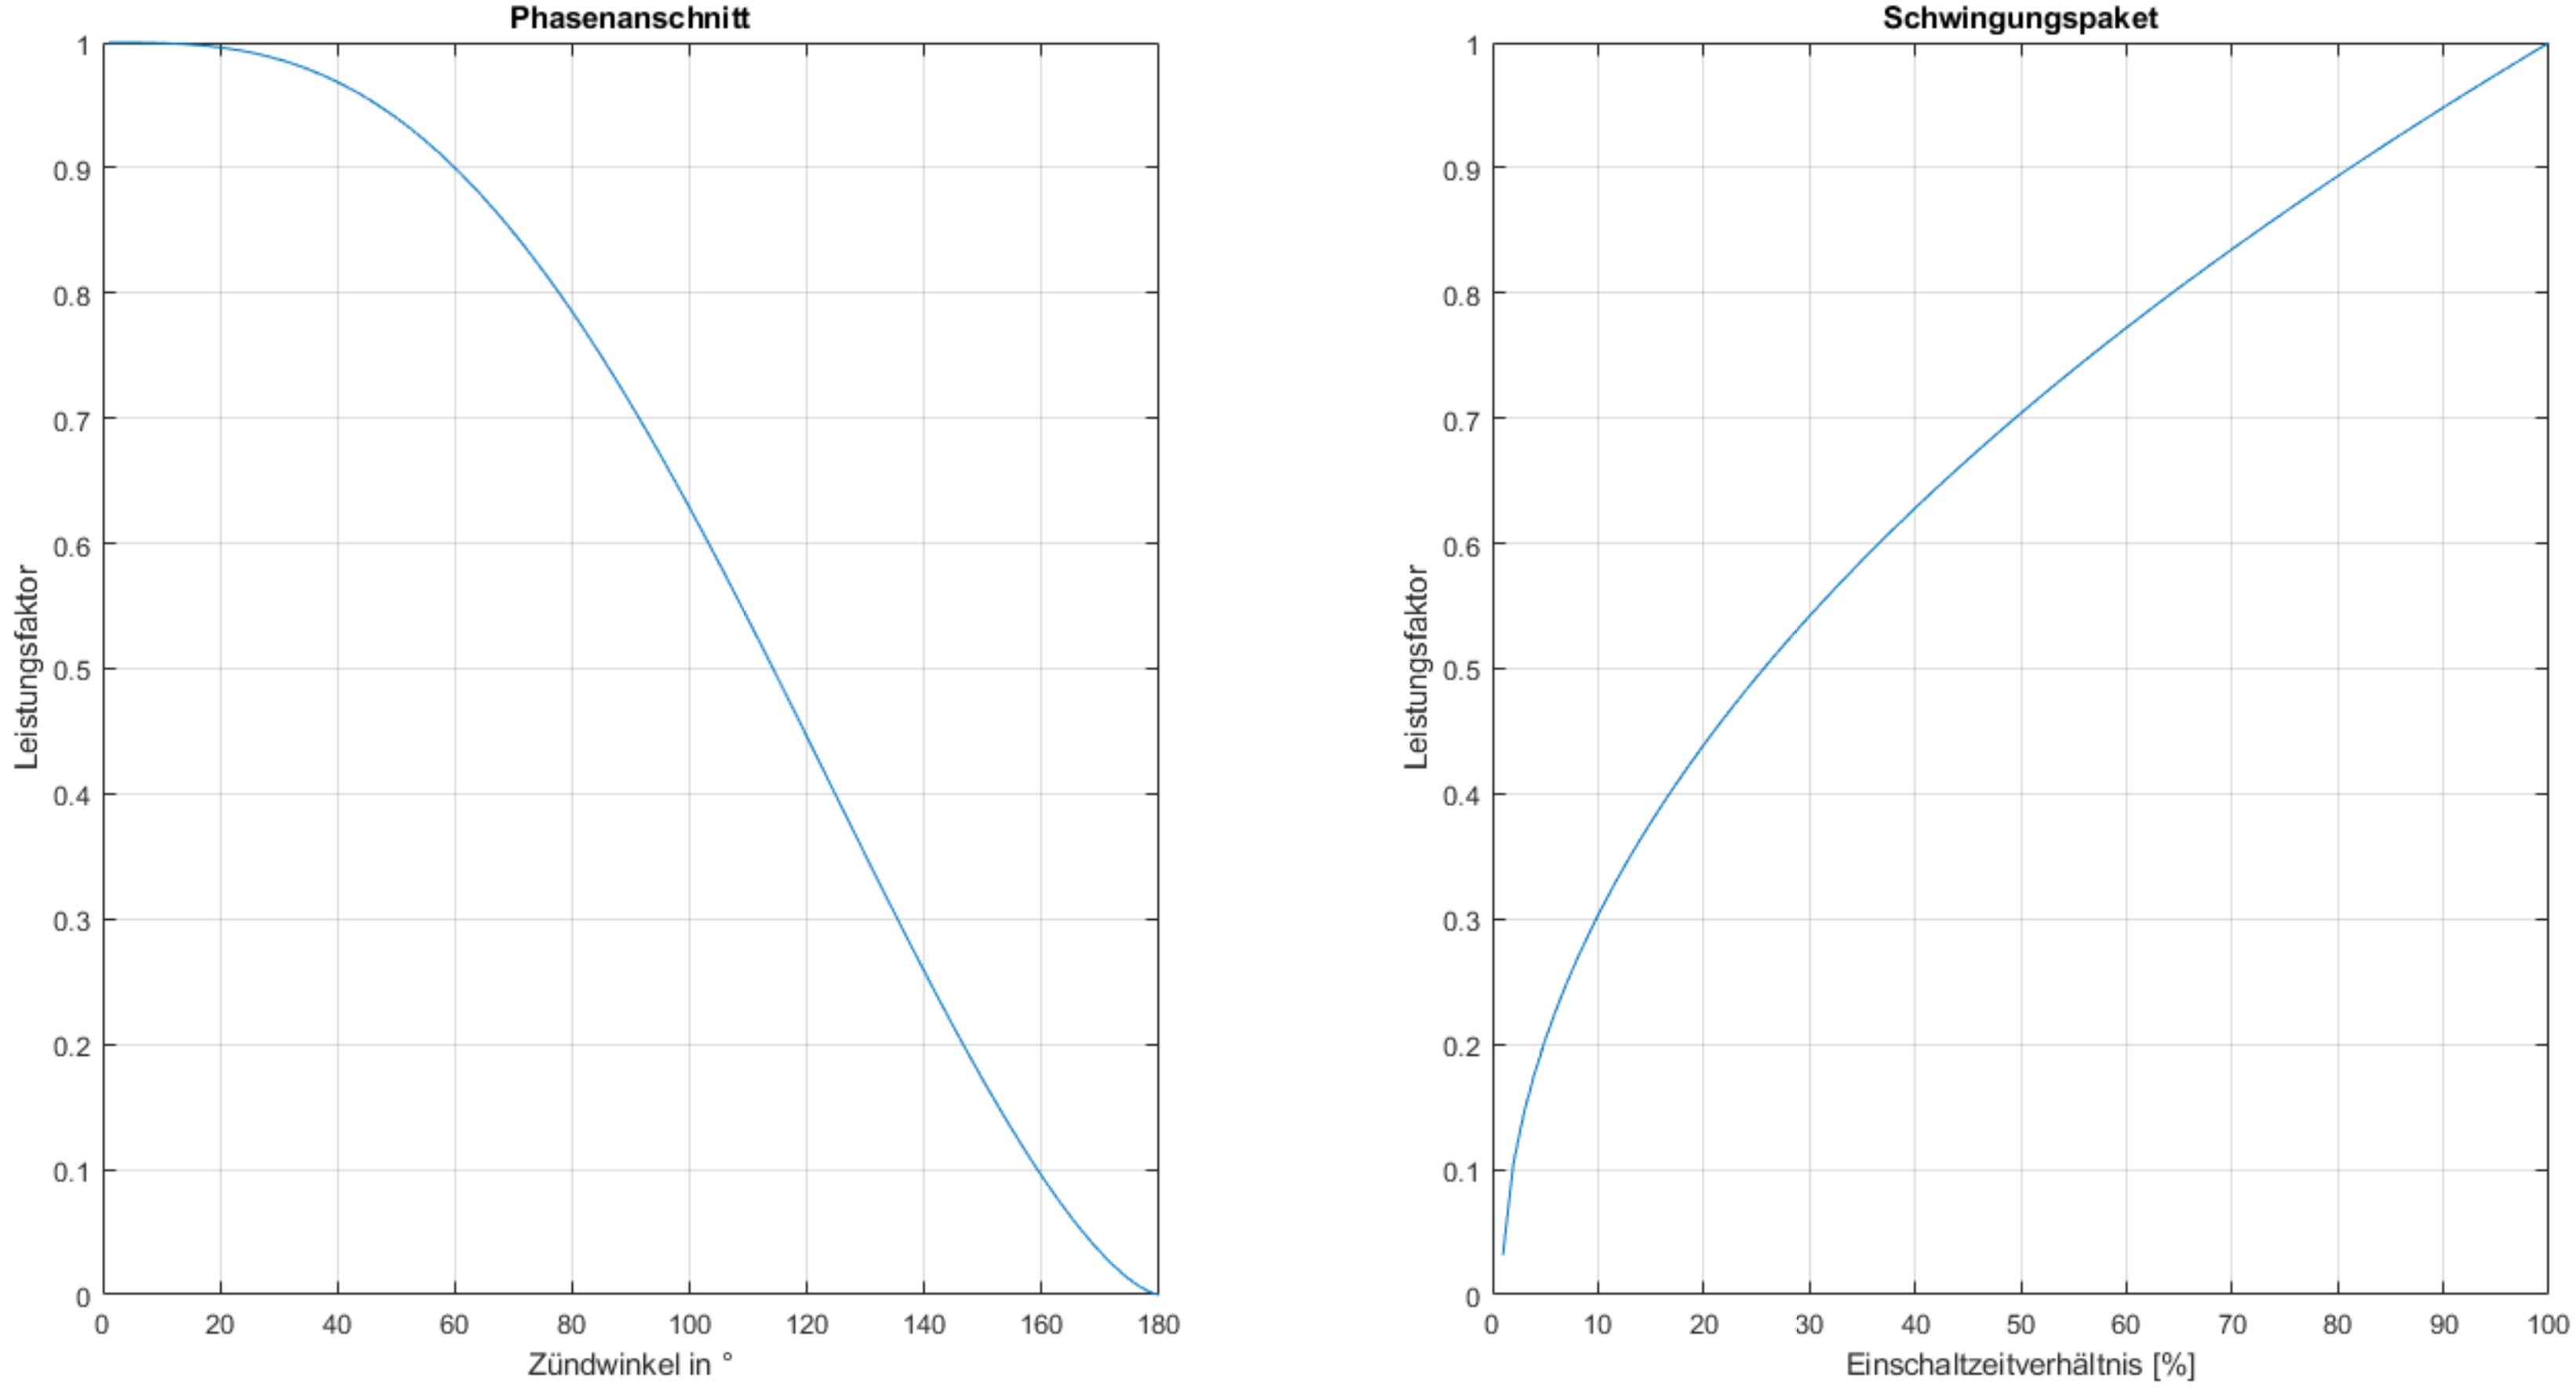
\includegraphics[scale=0.394]{Leistungsfaktor.png}	
	\caption{Leistungsfaktor von Phasenanschnitt- und Schwingungspaketsteuerung}\label{fig:Leistungsfaktor}
\end{figure}

\subsubsection{Leistungsfaktor Phasenanschnittsteuerung}
Der Leistungsfaktor ist definiert als das Verhältnis von Wirkleistung zu Scheinleistung. 
\begin{equation}\label{eq:lamda_p}
\lambda = \frac{P_{\alpha}}{S}
\end{equation}
Die Schein- und Wirkleistung können mit den folgenden Formeln beschrieben werden.
\begin{equation}\label{eq:Schein-&Wirkleistung}
\begin{array}{cc} 
S = I_L \cdot U_{UN}   &   P_{\alpha} = I_L^2 \cdot R_L  \\
\end{array}
\end{equation}
Werden die Formeln \ref{eq:Schein-&Wirkleistung} in die Formel \ref{eq:lamda_p} eingesetzt ergibt sich folgende Gleichung. 
\begin{equation} \label{eq:Phas_1}
\frac{P_{\alpha}}{S} = \frac{I_L \cdot R_L}{U_{UN}}
\end{equation}
Der Laststrom wird mit folgender Formel beschrieben.
\begin{equation}
I_L = \sqrt{1-\frac{\alpha}{\pi}+\frac{1}{2\pi} \cdot sin(2\alpha)} \cdot \frac{U_{UN}}{R_L}
\end{equation}
Wenn die Formel für den Laststrom in die Gleichung \ref{eq:Phas_1} eingesetzt wird, lassen sich die Spannung und der Widerstand wegkürzen und übrig bleibt folgende Formel.
\begin{equation}
\lambda = \sqrt{1-\frac{\alpha}{\pi}+\frac{1}{2\pi} \cdot sin(2\alpha)}
\end{equation}

\subsubsection{Leistungsfaktor Schwingungspaketsteuerung}
Das Einschaltsverhältnis wird mit $a$ beschrieben und wird mit der Formel \ref{eq:Einschaltverhältnis} beschrieben.
Die Schein- und Wirkleistung werden mit den folgenden Formeln beschrieben.
\begin{equation}\label{eq:Schw_Schein-&Wirkleistung}
\begin{array}{cc} 
S_a = \sqrt{a} \cdot P  &   P_a = a \cdot P \\
\end{array}
\end{equation} 
Wenn die beiden Formeln für die Wirk-und Scheinleistung in die Gleichung für den Leistungsfaktor eingesetzt wird ergibt sich daraus folgende Gleichung.  
\begin{equation}
\lambda = \frac{P_a }{S_a} = \frac{a \cdot P}{\sqrt{a} \cdot P}
\end{equation}
Die Wirkleistung lässt sich wegkürzen und so ergibt sich folgende Formel.
\begin{equation}
\lambda = \sqrt{a}
\end{equation}

\subsection{Oberschwingungen}
Im Idealfall würde bei einer Stromversorgung überall eine perfekte sinusförmige Spannung vorliegen. Jedoch sieht dies in der Realität anders aus. Die Kurve der Spannung und des Stromes weichen massiv von einer Sinusfunktion ab. Man bezeichnet diese verzerrten Schwingungsformen im Allgemeinen als oberschwingungsbehaftetes Signal. 

Schon früh erkannte man diese Oberschwingungsverzerrungen am Netz, jedoch ist es erst heute ein ernstzunehmendes Problem für die Versorgungsbetriebe, die Verteilnetzbetreiber und für den Endkunden. Früher waren die grössten Herausforderungen, die Auswirkungen von Oberschwingungsverzerrungen auf elektrische Maschinen zu erkennen. Man stellte ausserdem fest, dass Störungen in den Telefonleitungen auftraten die die Sprache störten. Allerdings kann man sagen, dass Oberschwingungsverzerrungen früher ein geringeres Gefahrenpotential darstellten als heute. Die heutigen Maschinen wurden neuerdings so konstruiert, dass sie weniger Oberwellen erzeugen. Auch bei den Verteilnetzen wurde darauf geachtet, dass sie nicht mehr an der Lastgrenze arbeiten. Seit einigen Jahren steigt, die weltweite Nachfrage nach energieeffizienten Lösungen, die nur über vermehrten Einsatz von Leistungselektronik realisierbar sind. 
\subsection{Grundlagen}
Die Bedeutung Oberschwingung kommt aus dem Themenbereich «physische Eigenwertprobleme» also Wellen, deren Frequenz ganzzahlige Vielfache der Grundschwingungen sind. In der Musikwelt kann man Oberschwingungsfrequenzen vor allem bei Saiteninstrumenten, wie zum Beispiel bei einer Gitarre oder einer Geige beobachten. Die meisten elektrischen Geräte halten sich nach der perfekten Welle Ausschau. Bei Wechselstrom bedeutet dies eine perfekte Sinuskurve. Die elektrische Spannung wechselt gleichmässig zwischen der positiven und negativen Halbwelle hin und her. Bei einer Frequenz von 50 Hz beträgt dies genau 50-mal pro Sekunde. Der Begriff Welle ist mit dem Zusammenhang von Oberschwingungen nicht ganz korrekt. Eine Welle hat eine räumliche und zeitliche Ausdehnung, jedoch haben die hier betrachteten Schwingungen nur eine zeitliche Ausdehnung. Die Oberschwingungsanteile in einem Wechselstromsystem sind also definiert als sinusförmige Anteile einer periodischen Schwingung, deren Frequenz einem ganzzahligen Vielfachen (Ordnungszahl) der Grundfrequenz entspricht. In der unteren Tabelle erkennt man welche Ordnungszahl oder auch genannt Oberschwingung zu welcher Frequenz gehört. Es ist veranschaulicht, dass zum Beispiel die 5. Oberschwingung eine Frequenz von 250 Hz hat.  

\begin{equation}
f_h = n \cdot Grundfrequenz
\end{equation}

\begin{table}[ht!]
	\centering
	\begin{tabular}{|l|l|}
		\hline
		\begin{tabular}[c]{@{}l@{}}Ordnungszahl\\   ($f_h$)\end{tabular} & \begin{tabular}[c]{@{}l@{}}Frequenz (Hz)\\   im Netz\end{tabular} \\ \hline
		1                                                             & 50                                                                \\ \hline
		3                                                             & 150                                                               \\ \hline
		5                                                             & 250                                                               \\ \hline
		7                                                             & 350                                                               \\ \hline
		11                                                            & 550                                                               \\ \hline
		13                                                            & 650                                                               \\ \hline
		\dots                                                         & \dots                                                             \\ \hline
		$n$                                                           & 								$50 \cdot n$                                                      \\ \hline
	\end{tabular}
\caption{Oberschwingungsfrequenz}
\end{table}

\begin{figure}[ht!]
	\begin{minipage}[t]{0.49\textwidth}
		\centering
		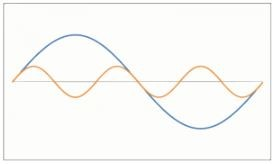
\includegraphics[scale=2]{Schwing_3.jpg}	
		\caption{Grundschwingung mit 3. Ordnung \cite{Oberwellen}}\label{fig:Schwing3}
	\end{minipage}	
		%
	\begin{minipage}[t]{0.49\textwidth}	
		\centering	
		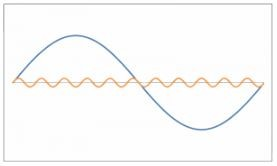
\includegraphics[scale=2]{Schwing_11.jpg}	
		\caption{Grundschwingung mit 11. Ordnung \cite{Oberwellen}}\label{fig:Schwing11}
	\end{minipage}
\end{figure}
	
Die folgenden zwei Abbildungen \ref{fig:Schwing3} \& \ref{fig:Schwing11} zeigen eine Grundschwingung bei 50 Hz (blau) und die jeweilige 3. und 11. Harmonische der Grundfrequenz (gelb).

\subsection{Verzerrte Schwingung}
Eine verzerrte Schwingung entsteht durch Überlagerungen von verschiedenen sinusförmigen Wellen mit unterschiedlichen Frequenzen und Amplituden. Man kann eine solche Schwingung mit unterschiedlichen Oberschwingungskomponenten, auch Komposition genannt, zusammensetzen, indem man eine Sinusschwingung mit mehreren Oberschwingungen zusammenaddiert. Das folgende wellenförmige verzerrte Signal lässt sich zu einer Grundschwingung mit ihren mehreren harmonischen Oberschwingungen zerlegen. Bei der untenstehenden Graphik \ref{fig:Addition Oberwellen} ist genau diese ersichtlich, wobei die rote Kurve das verzerrte Signal ist. Die blauen Sinusschwingungen sind die Zerlegungen in die Grundschwingung der 3. und 5. harmonische Oberschwingung. Addiert man wiederum die drei blauen Kurven miteinander erhält man das verzerrte rote Signal.   

\begin{figure}[ht!]
	\centering
	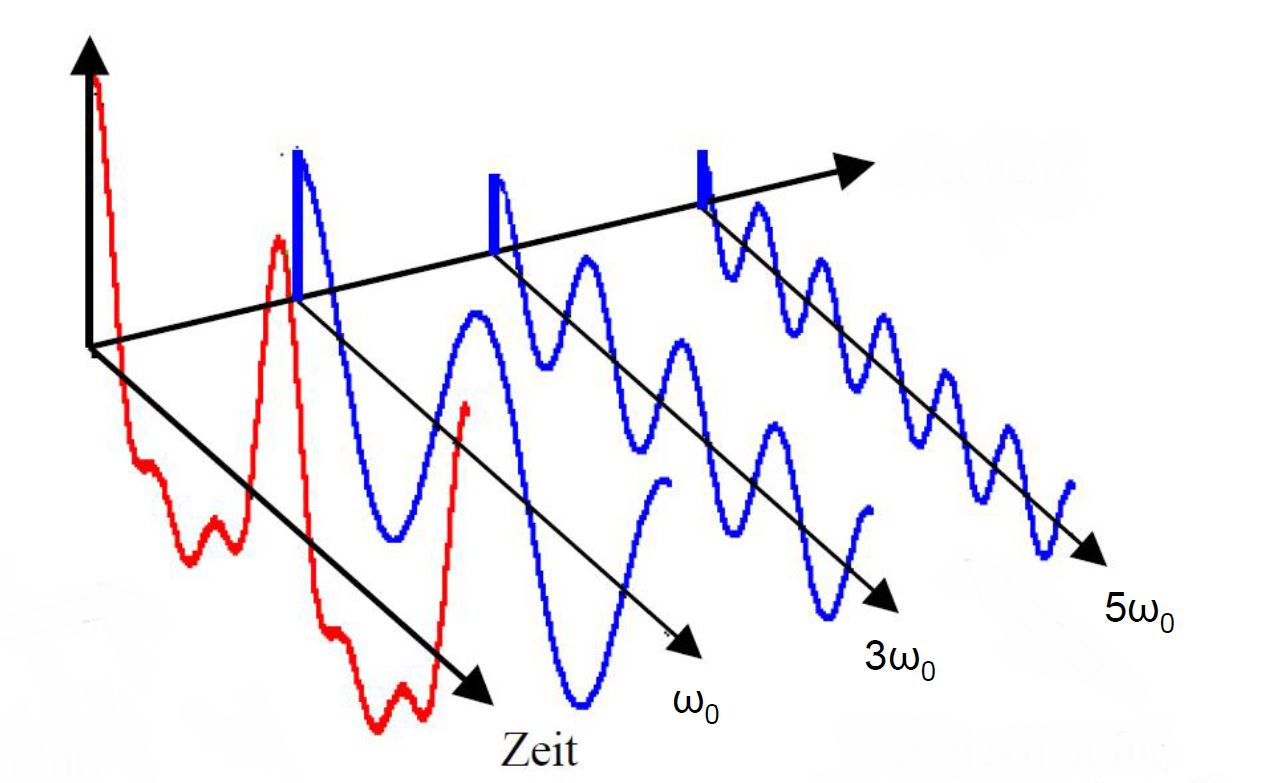
\includegraphics[scale=0.7]{verzerrtes_Signal_analysis.png}	
	\caption{Addition der verschiedenen Oberwellen \cite{analysi3}}\label{fig:Addition Oberwellen}
\end{figure}


Die erste Person, welcher diese Methode vorgestellt hat, war der französische Mathematiker Jean Baptiste Fourier. Noch heute trägt die Fourier-Transformation diese Bezeichnung. Mit diesem Zusammenhang kann die Überlagerung von einer perfekten Sinuskurve zu einer verzerrten Sinusschwingung führen. Dies Bedeutet so viel wie, eine verzerrte Sinusschwingung lässt sich immer als Überlagerung einer Grundschwingung mit anderen Oberschwingungen unterschiedlicher Frequenzen und unterschiedlichen Amplituden darstellen. Anhand eines Amplitudenspektrums lassen sich die Oberschwingungen gut visualisieren. 
\todo evt. noch Bild mit Amplitudenspektrum einfügen
Bei den Oberschwingungen handelt es sich um ungerade oder gerade harmonische Schwingungen.
Die ungeraden Oberschwingungen sind die charakteristischen Oberschwingungsanteile in den heutigen Stromversorgungsnetzen. Sie stellen Wellenformen dar die bezogen auf die Zeitachse symmetrisch sind. Aufgrund der meist dreiphasigen Symmetrie der heutigen Infrastrukturen sind nahezu alle Signale symmetrisch, obwohl es zu Verzerrung kommt. Geradzahlige Oberschwingungen können nur aus Wellenformen entstehen, die nicht symmetrisch bezogen auf die Zeitachse sind.

\subsection{Vorkommen der Oberschwingungen}
Oberschwingungsströme erzeuget fast jedes elektrische Gerät. Doch welches Gerät welche Stromverzerrung erzeugt wird später erklärt. Ein wichtiger Bezugspunkt zu den individuellen Oberschwingungsgrössen ist die gesamte harmonische Verzerrung. Man nennt ihn auch den THD-Wert (Total Harmonic Distortion). Diesen Wert gilt es besonders zu verstehen, damit man ihn Rechnerisch analysieren kann. Er gibt ausserdem das Verhältnis des Effektivwertes aller Oberschwingungen zum Effektivwert der Grundschwingung an. Er wird üblicherweise in Nieder-, Mittel-, aber auch im Hochspannungsnetz verwendet. Normalerweise wird die Verzerrung des Stromes als THDi beschrieben in der Formel \ref{eq:THDi} und die Verzerrung der Spannung als THDu beschriftet in der Formel \ref{eq:THDu} angegeben. Der Total Harmonic Current (THC) ist der gesamte Oberschwingungsstrom. Er wird verwendet, um den Gesamteffektivwert der Oberschwingungsströme der Ordnung 2 bis 40 zu quantifizieren, die zu einer Verzerrung der Stromkurve beitragen. Man erkennt dies in der Formel \ref{eq:THC}. Diesen Wert braucht man vor allem, um die erforderlichen Eigenschaften zur Auswahl eines effizienten aktiven Oberschwingungsfilters zu bestimmen.

Bei der folgenden Formel handelt es sich um den Gesamten Oberschwingungsstrom.
\begin{equation}\label{eq:THC}
THC = {\sqrt{\sum_{n=2}^{40} I_n^2}}
\end{equation}



Die gesamte harmonische Verzerrung des Stromes gibt, wie der Name schon sagt, die gesamte Verzerrung des Stromes an. Der Wert ist definiert als Quotient des Effektivwerts der Oberschwingungsströme im Verhältnis zum Grundschwingungsstrom. Typischerweise wird die Summe aller Stromoberschwingungsanteile in Bezug auf den Grundschwingungsstrom bis einschliesslich der 40. Oberschwingung berechnet. Die Oberschwingungsströme, welche durch Lasten in Netzwerken erzeugt werden, müssen durch die Impedanzen der Transformatoren oder Drosseln fliessen. An diesen Impedanzen kommt es zu nichtlinearen Spannungsabfällen. Es werden Oberschwingungsspannungen erzeugt die im ganzen Netz verbreitet werden. Diese können an Endgeräten eine Verzerrung der Versorgungsspannung verursachen. Somit ist die harmonische Verzerrung des Stromes (THDi) eine direkte Ursache für die Verzerrung der Spannung (THDu = Total Harmonic Distortion of Voltage). Sie gibt das Ausmass der Verzerrung der Versorgungsspannung an. Auch dieser Wert ist definiert als Quotient des Effektivwertes der Spannungsoberschwingungsanteile bis zur 40. Oberschwingung bezogen auf den Effektivwert der Grundschwingung. 

Folgende Formel zeigt wie man die Totale Verzerrung des Stromes in Prozent berechnet ist.
\begin{equation}\label{eq:THDi}
THDi = \frac{\sqrt{\sum_{n=2}^{40} I_n^2}}{I_{(1)}} * 100 \%
\end{equation}

Parallel dazu zeigt die untere Formel die Totale Verzerrung der Spannung in Prozent.
\begin{equation}\label{eq:THDu}
	THDu = \frac{\sqrt{\sum_{n=2}^{40} U_n^2}}{U_{(1)}} * 100\%
\end{equation}






Je niedriger der THDu-Wert ist, desto besser ist die Spannungsqualität. Die Norm besagt, dass der gesamte Oberschwingungsgehalt den Wert von 8\% nicht überschreiten darf. Dazu kommt, dass heute üblicherweise für die Verzerrung die THD-Werte angegeben sind und nicht wie früher die Oberschwingungsgehalte (Klirrfaktore).

Wenn man sich mit den Oberschwingungsproblematik befasst, ist es wichtig, den Zusammenhang zwischen Strom und Spannung zu verstehen. Dadurch ist es möglich eine geeignete Lösung für das reduzieren von Oberschwingungen zu finden. 
Je nach Eigenschaft der Oberschwingungserzeuger und der Eigenschaft eines Gerätes am elektrischen Netz, verbreiten sich Oberschwingungsströme in einem System unterschiedlich. Verschiedene Spannungsverzerrungen sind die Folgen. 

\subsection{Auswirkung von Oberschwingungen}

Falls Oberschwingungen oder andere Netzrückwirkungen bei Betriebsmitteln auftreten, können die Funktionen von den Geräten beeinträchtigt oder sogar zerstört werden. Ein Beispiel dafür wäre, im Falle einer Kurzzeitunterberechnung bei Schaltnetzteile würden sie mit extrem hohen Einschaltspitzen reagieren. Diese Spitzen könnten das 20-fache der Nennlast erreichen. Im einphasigen Verbrauch in einem Dreiphasigen-Wechselstromsystem fliesst der ganze Rückleitstrom über den Sternpunkt des Transformators zurück. Gäbe es viele Schaltnetzteile in einem System, würden sich die Rückleiterströme nicht mehr aufheben, sondern sie würden sich addieren. Die Folgen davon wäre eine Sternpunktverschiebung. Oberschwingungen können bei Glühbirnen die Glühfadentemperatur erhöhen und somit die Lebensdauer verkürzen. Auch bei Dreh- oder Wechselstrommotoren und -generatoren führen Stromoberschwingungen zu zusätzlicher Erwärmung. Bei Schutzgeräten wie Distanzschutz, Überstromschutz oder Differentialschutz können Oberschwingungen den Aufbau und die Wirkungswiese des Schutzgerätes beeinflussen. Sind die Abstände zwischen Freileitungen und Telefonleitungen zu gering, können die Oberschwingungen die Sprachübertragung stören. Dabei gibt es vor allem ein Auge auf die 20. bis zur 30. Ordnung der Oberschwingung zu werfen.

\subsection{Anforderung an die Netzqualität}

Um die Anforderungen der Netzqualität zu gewährleisten müssen die Normen eingehalten werden. Auf welche Nomen bei dieser Arbeit genau geachtete wurde, wird zu einem späteren Zeitpunkt erläutert. Zweck der Normen sind es  die verschiedene Merkmale wie zum Beispiel Frequenz, Höhe, Kurvenform oder die Symmetrie der drei Leiterspannungen einzuhalten. Durch Lastspannung, Störeinflüsse von bestimmten Anlagen oder Auftreten von Fehlern können diese Merkmale während des Normalbetriebes des Netzes geändert werden. 


\subsection{Gegenmassnahmen bei Oberschwingungen}

Es kann durchaus vorkommen, dass in der Praxis harmonische Oberschwingungen festgestellt wurden, welche die zulässigen Grenzwerte überschreiten. Es gibt jedoch Möglichkeiten diese zu verhindern und so die Netzqualität zu verbessern. Im folgenden Abschnitt werden auf ein paar Varianten eingegangen.

\subsubsection{Vermeidung von Störungen}
Das Vermeiden von Störungen ist die einfachste Art um eine Verbesserung der Netzqualität sicher zu stellen. Der Gesetzgeber liefert dafür Normen der Elektromagnetischen Verträglichkeit, welche den gesetzlichen Grundlagen entsprechen. Sie sind zwingend einzuhalten.
\subsubsection{Stromnetzeigenschaften}
Könnte man die Netzimpedanz verringern wäre eine Reduktion der Oberschwingungen möglich. Dies ist jedoch generell nicht umsetzbar und somit kann man Kurzschlussleistung des Netzes nicht beliebig erhöhen. Die wirtschaftlichen und technischen Grenzen sind hierzu massgebend.  


\subsubsection{Oberschwingungsfilter}

Zur Begrenzung von Oberschwingungen werden heutzutage  meistens mehrere aufeinander abgestimmte passive Filter eingesetzt. Das einsetzten von den Filtern muss jedoch für jede konkrete Installation neu erstellt werden um eine Verbesserung des Netzrückwirkungsverhaltens zu erhalten.\\
Die Industrie entwickelte genau wegen diesem Problem aktive Oberschwingungsfilter. Sie können sich, auch bei späteren Erweiterungen der Installation, an die neu Situation angepasst werden und müssen nicht ersetzt werden. Ein weiterer Vorteil dieser Flexibilität des Filters ist es, dass die Nenngrösse einfach vom aktuellen Bedarf gewählt werden kann.     

\subsubsection{Änderung der Energieversorgung}

Stark nichtlineare Betriebsmittel und empfindliche Verbraucher die zusammen an einer Gruppe angeschlossen sind, können aufgetrennt und an separate Gruppen über jeweils einen separaten Transformator eingespeist werden. Eine solche Änderung der Energieversorgung sollte aber auch immer unter wirtschaftlichen Gesichtspunkten betrachtet werden.

\subsubsection{EMV verträgliche Gebäudeinstallation}

Um Schäden durch Oberschwingungen zu vermeiden müssen bei Gebäuden die Installation EMV-verträglich sein.
Folgende Punkte sollten dabei zwingend beachtet werden:

\begin{itemize}
	\item Es sollte ein konsequentes TN-S-Netz mit getrenntem Neutral- und Schutzleiter aufgebaut werden. Die beiden Leiter sollten nur eine Verbindung zwischen einem Punkt haben.
	\item Um Schäden an einer Anlage zu vermeiden wäre ein Überspannungsschutz für Kompensationsanlagen von Vorteil.
	\item Wie schon erwähnt, wären getrennte Stromkreisgruppen für allgemeine und IT-Betriebs-mittel vorteilhaft.
	\item Leitende oder metallene Teile, wie zum Beispiel Trasse, Rohre oder Lüftungskanäle sollten zwingend mit dem Potentialausgleich verbunden werden.
	
\end{itemize}

Auch die Energieversorgung bei der Gebäudeinstallation sollte EMV-verträglich sein. Folgende Punkte sollten dabei eingehalten werden. 

\begin{itemize}
	\item Das Erdungssystem sollte niederohmig und stromfähig installiert sein.
	\item Im Schutzleiter- und Potenzialausgleich-Systeme sollten keine Arbeitsströme zugelassen sein.
	\item Bei Mehrfacheinspeisung dürfen keine MEhrfacherdung des Neutralleiters zugelassen werden.
	\item Der Kabelquerschnitt sollte für die Oberschwingungen zugelassen sein.
\end{itemize}  


\subsubsection{Harmonische Oberwellen}
Um die einzelnen Vor- und Nachteile besser verstehen zu können, muss weiter erklärt werden, was die harmonische Oberwellen sind und wie sich diese im Netz verhalten.
\subsubsection{Subharmonische}
Da nicht nur harmonische Oberwellen verglichen werden, werden hier noch die Subharmonische erklärt und was der Unterschied zu den harmonischen Oberwellen ist. 
\subsubsection{Fast Fourier Transformation}
Damit die beiden Spektren der Oberwellen verglichen werden können, wird diese in einem FFT Diagram aufgezeigt. Wie diese zu lesen sind und was sie aussagen, wird hier beschrieben. 

\subsection{Total Harmonic Distortion}
Um die beiden Steuerungsarten vergleichen zu können, wird der THD benötigt. Wie dieser berechnet wird, wird in diesem Kapitel aufgezeigt. 
\todo{Andere Kapitel rauslöschen? Oder Titel anpassen}


\subsection{Normen}

